\chapter{Implementation}\label{ch:implementation}

\section{Different Spaces of Design Exploration}

The optimization of the LATOME firmware can be done by leveraging different division multiplexing approaches, HLS directives or design implementations. These are three different spaces of design exploration that were explored to improve the firmware. This chapter will present the different explorations that were conducted in the context of this thesis in a first section. Next, the second section will focus on the results obtained after testing these different options.

%%%%%%%%%%%%%%%%%%%%%%%%%%%%%%%%%%%%%%%%%%%%%%%%%%%%%%%%%%%%%%%%%%%%%%%%%%%%%%%%
%%%%%%%%%%%%%%%%%%%%%%%%%%%%%%%%%%%%%%%%%%%%%%%%%%%%%%%%%%%%%%%%%%%%%%%%%%%%%%%%
%%%%%%%%%%%%%%%%%%%%%%%%%%%%%%%%%%%%%%%%%%%%%%%%%%%%%%%%%%%%%%%%%%%%%%%%%%%%%%%%

\section{Methodology}

\subsection{Time Division Multiplexing}

The v5 of the LATOME firmware only uses the TDM approach. The data frames are broken down in different words which are processed sequentially. On the other hand, the v6 firmware leverages almost only the SDM approach with parallel interfaces for the ISM and OSUM blocks, using deserializer and serializer.

As the base code for this thesis is the v6 HLS firmware, the TDM design space can be explored by moving up or down the serializer currently placed at the output of the OSUM. The figure \ref{fig:slider-serializer} shows the different possible positions for the serializer. 
% Since the v6 Output Summing logic is almost only a combinational one, and processes parallel data, its clock can use any frequency above the \(40\)MHz one of the Bunch Crossings.

\begin{figure}
    \centering
    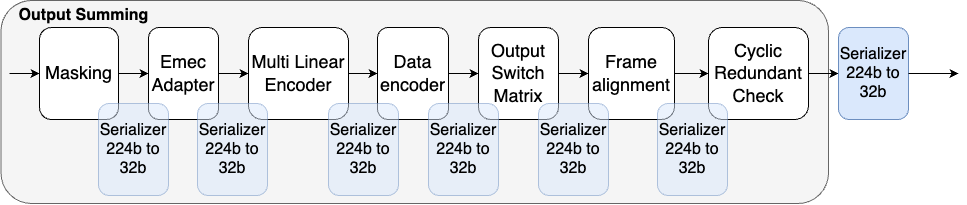
\includegraphics[width=1\textwidth]{slider_serializer.png}
    \caption{Current and potential positions of the serializer}
    \label{fig:slider-serializer}
\end{figure}

The serializer at the output of the OSUM breaks down frames of 224 bits into 7 words of 32 bits. The main intuition behind this design exploration is that using smaller data words could reduce the size of some design blocks. Meanwhile, the latency of the design remains unchanged, as the serializer is only moving up in the design.

During this thesis, the serializer was moved up to two main different positions. The first one was before the Output Switch Matrix, and the second one was before the Data Encoder. In both cases, the OSM, Frame Alignment and CRC9 blocks were modified to handle the new data format. 

An important aspect to check is the data dependencies, since these could have a critical impact when using TDM. The OSM block is a routing block which does not change any data in the frames. The Frame Alignment only overwrites the data that it gets as input if the current BC index is an alignment one, hence it does not show data dependencies. Finally the Cyclic Redundant Check can be both computed in a parallel or serial fashion equivalently and only depends on the CRC temporary result from time \(t=-1\). Having no data dependencies, the TDM approach can be used without any issue.

The new design of these blocks required little code changes but introduced new sequential logic, like counters, to keep track of the current word being processed. Additionally, the operating frequency becomes \(7\times40=280\)MHz, as the serializer must process 7 words of 32 bits in 7 clock cycles and the OSUM must maintain a throughput of 7 clock cycles to never miss new data from the detector.

\subsubsection{Output Switch Matrix}

The different LATOME boards must route the data differently to the FEX systems depending on the detector region they are connected to. To tackle this problem, either each LATOME has a different version of the firmware, or some code must be added to allow an online configuration procedure defining the routing. The second possibility was chosen in the LAr group, and the solution proposed by Marcos for the v6 firmware was to add an Output Switch Matrix. 

The OSM uses multiplexers to route the 17 inputs to the 48 outputs and takes its selection bits from registers configured online via an ipbus. The HLS implementation is very simple, involving a 2D array with 48 rows made of a subgroup of the 17 possible inputs.

\begin{figure}
    \centering
    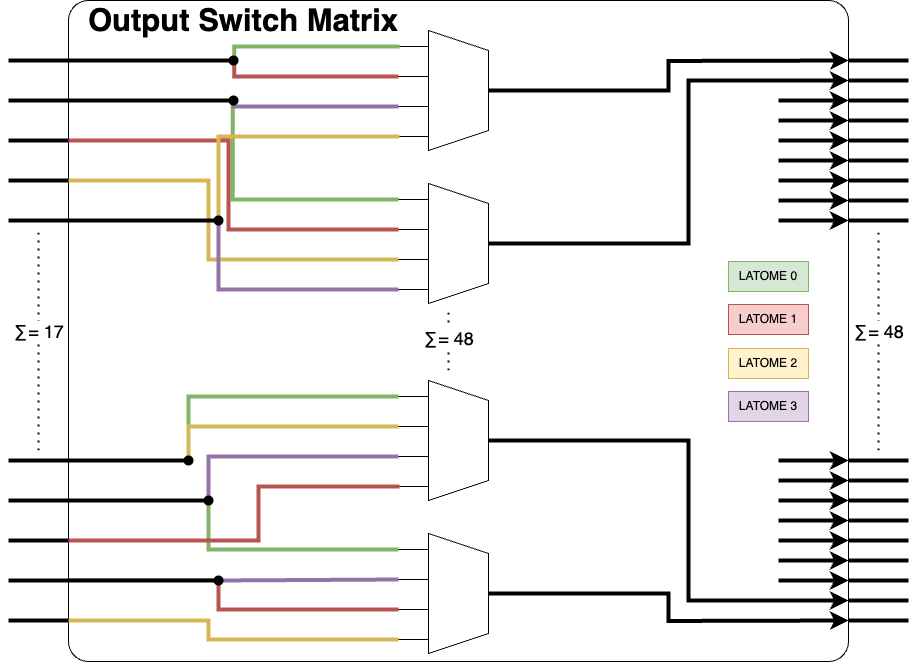
\includegraphics[width=0.6\textwidth]{osm.png}
    \caption{Output Switch Matrix Simplified Diagram}
    \label{fig:osm-design}
\end{figure}

Without looking at the different LATOME routings, it appears that, there should be 48 multiplexers of input size \(224\times17=3808\) bits. However when considering the data paths and optimizing for them, the biggest multiplexers turn out to have at most 4 input frames, meaning that each row from the HLS 2D array has only 4 entries. In other words, the Output Switch Matrix is a sparse matrix. By moving the serializer before the OSM, the biggest multiplexers have an input size of \(4\times32\) instead of \(4\times224\).

\subsubsection{Frame Encoder}

The frame encoder block is responsible for creating the 17 frames of 224 bits representing the whole data. When using parallel data, the block is very simple and only needs to concatenate and order the different data words. Serializing before the Frame Encoder, makes the building of 224 bits frames unnecessary.

The Frame Encoder takes as input the 320 MLE results, the control bits and the BCID and assembles them. To create the 32 bit words, a counter is used to keep track of the current word being processed. A ``switch'' statement is used to handle the different cases.

% The input energy levels are placed in the frames in a specific order, not following their array indexing, making the HLS code complex to write. The synthesis 

\subsubsection{Impact on the Following Blocks}

The seven sequential cycles needed to process the serial words making up one frame are created using a simple for loop without catapult unroll directives. The frame alignment and CRC9 blocks use a counter to keep track of the current word being processed. In the case of the CRC9, since the code is appended on the 9 last bits of the frames, the block must first compute 6 32-bit word followed by one 23-bit word. The overhead of having two specialized blocks is considered to be very small as each of them only contain a limited number of XOR gates.

The frame alignment block reads the current BC index and if it matches the alignment index, it overwrites the data with the new data, otherwise it simply forwards it. The introduction of a simple counter indicating which of the 7 words is currently being processed together with a ``switch'' statement taking care of the different cases is enough to get a TDM version of this block. Additionally, this block sends a 4 bit control character indicating for each byte if it is a data byte or a control byte. Before the serialization, the block sent the complete 28-bit control word, now it sends 4 bits at a time.


\subsection{Leveraging HLS Directives}

The second space of design exploration is the HLS directives, specifically, the CCORE related ones. Each processing block of the Output Summing is declared as a CCORE one. This makes Catapult optimize the design inside of the CCORE once to reuse it for all the instances. The two options offered by Catapult (sequential or combinational) were tested for each block.

Additionally, Catapult gives the possibility to set the design goal for the optimization to be either latency or area. Setting this goal to either one will have an important impact on the final result.

Overall, there are six different blocks with each two options for the CCORE and two options for the optimization goal. This gives a total of 128 different possible combinations. The table \ref{tab:ccore-optimization} shows the different possible combinations. The CRC9 block is not included as it is, by essence, a sequential block, and cannot be set as combinational.

\begin{table}[ht]
    \centering
    \begin{tabular}{|c|c|c|}
        \hline
        & Option & Value \\
        \hline
        \hline
        CCORE & 
            \begin{tabular}{@{}c@{}}
                Masking \\
                Emec Adapter\\
                MLE\\
                Data Encoder\\
                OSM\\
                Frame Alignment\\
            \end{tabular} &
            \begin{tabular}{c}
                Sequential / Combinational \\
                Sequential / Combinational \\
                Sequential / Combinational \\
                Sequential / Combinational \\
                Sequential / Combinational \\
                Sequential / Combinational \\
            \end{tabular} \\
        \hline
        \multicolumn{2}{|c|}{Optimization Goal} & Latency / Area \\
        \hline
    \end{tabular}
    \caption{Possible values for each HLS option}
    \label{tab:ccore-optimization}
\end{table}

In the OSUM, many ``for'' loops are used to create the different instances of the blocks. A full unroll means that the for loop creates as many parallel instances as there are iterations. In some cases, a partial unroll can be used to create a fixed number of instances which are reused to process all the data. For example a for loop of 320 iterations can have an ``unroll 4'' directive to create 4 instances that will process 80 iterations each. This can lead to very high area reduction at the price of latency. The choice of full or partial unroll can be done manually, or left to Catapult to decide. For this design exploration, we have given Catapult the freedom to choose the best unroll factor, within the following constraints:
\begin{itemize}
    \item The initiation interval (throughput) must be 7 clock cycles.
    \item The maximum latency is 26 clock cycles.
\end{itemize}
The first value is a direct consequence of the 280MHz operating frequency, while the second value is the latency of the v5 design, which should not be exceeded.

To create all the different combinations, a tcl script looping through each of them and launching the Catapult synthesis was used. The results were then analyzed to find the best combination of options. A follow-up Quartus compilation analysis was done to get more precise and meaningful results. Overall, the HLS synthesis run time for all the combination lasted around 9 hours, while the Quartus compilation for all the combinations lasted 3 days.

\subsection{Unrolling Inside or Outside the CCORE}

When developing the HLS code for these design blocks, two options can be considered using CCOREs in for loops, as illustrated in figure \ref{fig:unrolling-inside-outside}. The first one is to set the OSM, Frame Alignment or CRC9 as an elementary block processing only one frame at a time, and to create as many copies as there are frames to process. The second option is to make the design block process all the frames, and to set it as a CCORE. Using the HLS jargon, the first option refers to \textit{unrolling} ``outside'' of the CCORE, while the second refers to \textit{unrolling} ``inside'' of the CCORE.

\begin{figure}
    \centering
    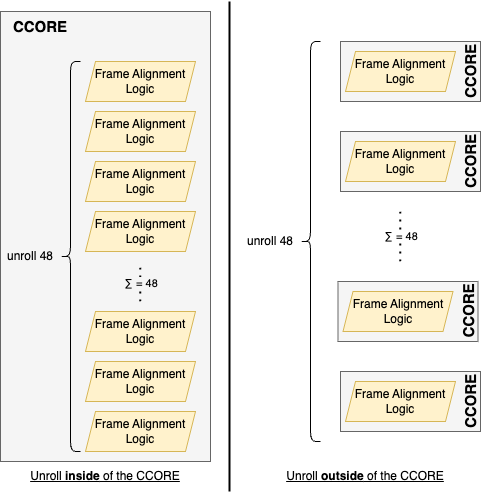
\includegraphics[width=0.6\textwidth]{unroll_inside_outside.png}
    \caption{Unrolling inside vs outside the CCORE}
    \label{fig:unrolling-inside-outside}
\end{figure}

For this DSE, the Frame Alignment and CRC9 blocks were considered. The study was performed by either using the creating the unrolled for loop in the CCORE or outside of it. The results were then compared to see which option was the best, both in the v6 firmware and in the new one.

%%%%%%%%%%%%%%%%%%%%%%%%%%%%%%%%%%%%%%%%%%%%%%%%%%%%%%%%%%%%%%%%%%%%%%%%%%%%%%%%
%%%%%%%%%%%%%%%%%%%%%%%%%%%%%%%%%%%%%%%%%%%%%%%%%%%%%%%%%%%%%%%%%%%%%%%%%%%%%%%%
%%%%%%%%%%%%%%%%%%%%%%%%%%%%%%%%%%%%%%%%%%%%%%%%%%%%%%%%%%%%%%%%%%%%%%%%%%%%%%%%

\section{Design Space Explorations Results}

To get results from a specific optimization, one can compile only the block being studied, the block within its parents block, or the whole firmware. In the LATOME HLS team, four levels of compilation exist and can be considered in this thesis: the block alone, within the OSUM, with the ISM and finally the whole firmware. Improvements on one level does not necessarily translate to the next as Quartus may or may not be able to perform further optimizations. However, at each level, the results can be compared to the original design to get a sense of the impact of the optimization. Additionally, the smaller compilation times of the lower levels can be used to quickly test different options.

%%%%%%%%%%%%%%%%%%%%%%%%%%%%%%%%%%%%%%%%%%%%%%%%%%%%%%%%%%%%%%%%%%%%%%%%%%%%%%%%
%%%%%%%%%%%%%%%%%%%%%%%%%%%%%%%%%%%%%%%%%%%%%%%%%%%%%%%%%%%%%%%%%%%%%%%%%%%%%%%%

\subsection{Time Division Multiplexing}

%%%%%%%%%%%%%%%%%%%%%%%%%%%%%%%%%%%%%%%%%%%%%%%%%%%%%%%%%%%%%%%%%%%%%%%%%%%%%%%%

\subsubsection{Serializing Before the OSM}

The expected results at the block level are an increase of the maximum operating frequency, as less signals must be synchronized, as well as an area reduction of a factor of 7.

\begin{table}[ht]
    \centering
    \begin{tabular}{|c|c|c|}
        \hline
        Version & Area (ALMs) & \(F_{max}\) (MHz) \\
        \hline
        Original OSM & 3621.5 & 310.17 \\
        Serialized OSM & 476.8 & 524.38  \\
        \hline
        Improvement & \(-86.8\%\) & \(+69.1\%\) \\
        \hline
    \end{tabular}
    \caption{Results From the OSM Optimization}
    \label{tab:osm-optimization}
\end{table}

The table \ref{tab:osm-optimization} shows an actual area reduction of a factor of 7.6 and an increase of the maximum operating frequency of 69\%. The area reduction is slightly higher than the expected factor of 7, which can be explained by the overhead that the signal synchronization logic had on the original design. 

%%%%%%%%%%%%%%%%%%%%%%%%%%%%%%%%%%%%%%%%%%%%%%%%%%%%%%%%%%%%%%%%%%%%%%%%%%%%%%%%

\subsubsection{Serializing Before Frame Encoder}

%%%%%%%%%%%%%%%%%%%%%%%%%%%%%%%%%%%%%%%%%%%%%%%%%%%%%%%%%%%%%%%%%%%%%%%%%%%%%%%%
%%%%%%%%%%%%%%%%%%%%%%%%%%%%%%%%%%%%%%%%%%%%%%%%%%%%%%%%%%%%%%%%%%%%%%%%%%%%%%%%

\subsection{HLS Directives}

Once the results were obtained, they were extracted in an Excel file to be analyzed. A python script created the different figures presented in this section. 

The first figure, figure \ref{fig:dse-overall}, shows the overall results for all the combinations, each represented by a point. The color of the points indicate the latency for this solution. Finally, the blue horizontal line shows the operating frequency of the OSUM block, 280MHz. This figure shows that the solutions with the highest latencies are the ones with the worst \(F_{max}\). This is explained by the fact that when Catapult implements resource sharing, with partial unrolling, the latency increases, but the resource sharing logic has a negative impact on the \(F_{max}\).

In figure \ref{fig:dse-goal}, the points are ``+'' when the goal for the solution is latency and ``o'' when it is area. Each line connects two solutions with all the same options except for the optimization goal. The line colorization depends on the latency. For instance, the points on the left of the figure all have lines going from bottom left to top right, with a color gradient from red to yellow. Additionally, the points at the bottom left are all area optimized solutions, while the ones at the top right are latency optimized solutions. This indicates that using the latency optimization goal will lead to a higher \(F_{max}\), lower latency at a small area cost, since the lines have a very big slope. Two clusters can be clearly distinguished, the one on the left showing a clear tendency and the one on the right showing a more scattered distribution.

Figures \ref{fig:dse-ena-mux}, \ref{fig:dse-emec-adapter}, \ref{fig:dse-efex-data}, show no clear tendency when varying the CCORE type for the Masking, EMEC Adapter and Data Encoder blocks. These blocks are more secondary ones for the optimizations and are very dependent on the more important ones. Hence they should be used for adjustments once the main blocks are optimized.

The figures \ref{fig:dse-efex-mle}, \ref{fig:dse-osm}, \ref{fig:dse-frame-select} show the results when varying the CCORE type for the MLE, OSM and Frame Select blocks. The MLE block shows a clear tendency: all the points on the right are combinational ones, while the ones on the left are sequential, the lines have a very small slope, and points are far from each other. This means that setting the MLE CCORE as sequential instead of combinational has a small impact on the \(F_{max}\), but reduces the area drastically. The OSM has almost no impact on the area, since the lines are vertical, but has one on the \(F_{max}\), which is very dependant on the other blocks' settings. Finally, most of the lines for the Frame Select block are going from the bottom right where the combinational points are to the sequential ones on the top left, indicating that the sequential setting has a positive impact both on the \(F_{max}\) and the area.

\begin{figure}
    \centering
    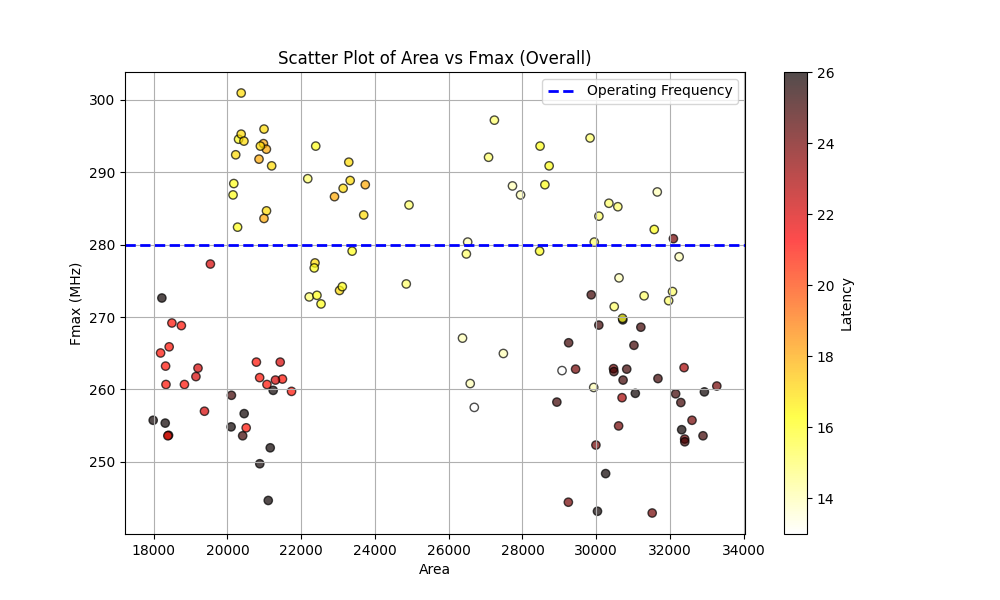
\includegraphics[trim={1cm 0 3cm 0}, clip, width=1\textwidth]{dse_overall.png}
    \caption{Overall Results}
    \label{fig:dse-overall}
    \centering
    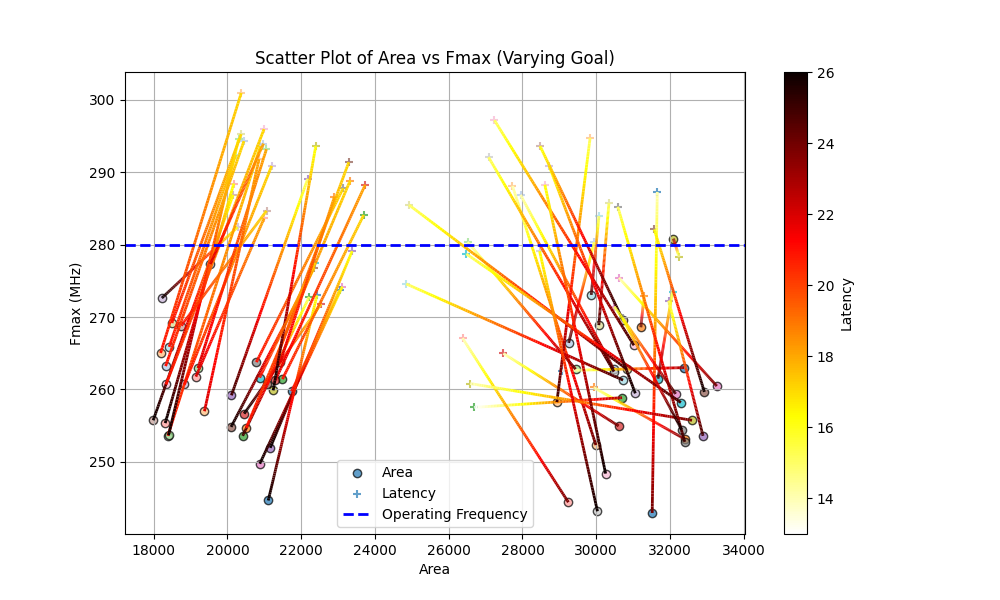
\includegraphics[trim={1cm 0 3cm 0}, clip, width=1\textwidth]{dse_goal.png}
    \caption{Results when varying the design goal}
    \label{fig:dse-goal}
\end{figure}
\begin{figure}
    \centering
    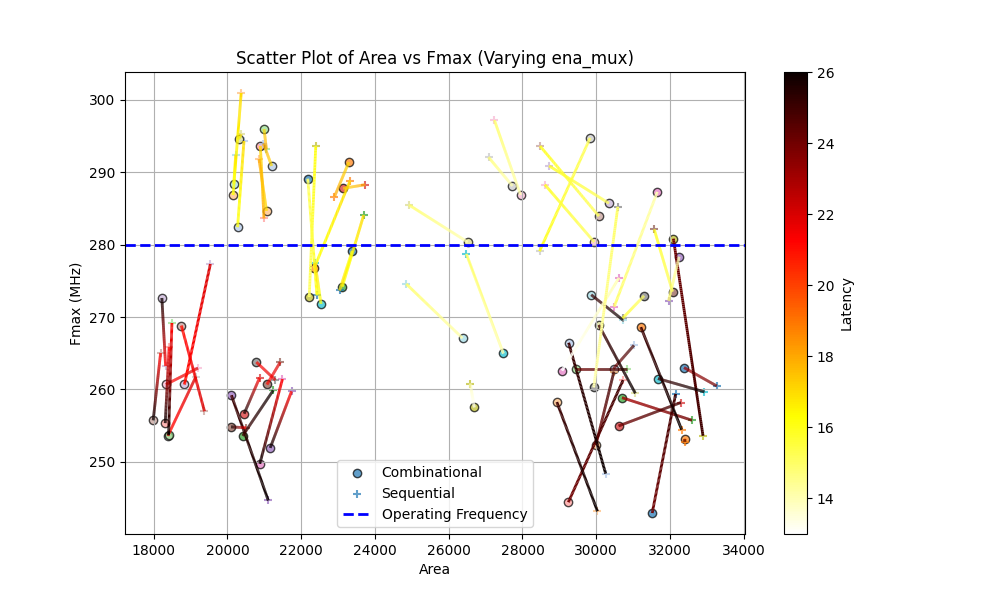
\includegraphics[trim={1cm 0 3cm 0}, clip, width=1\textwidth]{dse_ena_mux.png}
    \caption{Results when varying the CCORE type for the Masking}
    \label{fig:dse-ena-mux}
    \centering
    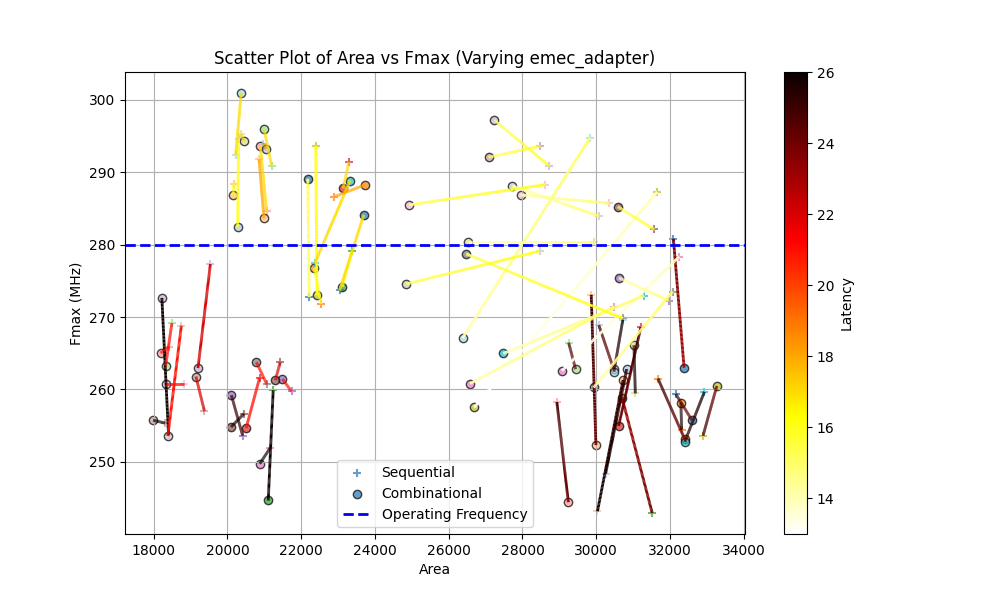
\includegraphics[trim={1cm 0 3cm 0}, clip, width=1\textwidth]{dse_emec_adapter.png}
    \caption{Results when varying the CCORE type for the EMEC Adapter}
    \label{fig:dse-emec-adapter}
\end{figure}
\begin{figure}
    \centering
    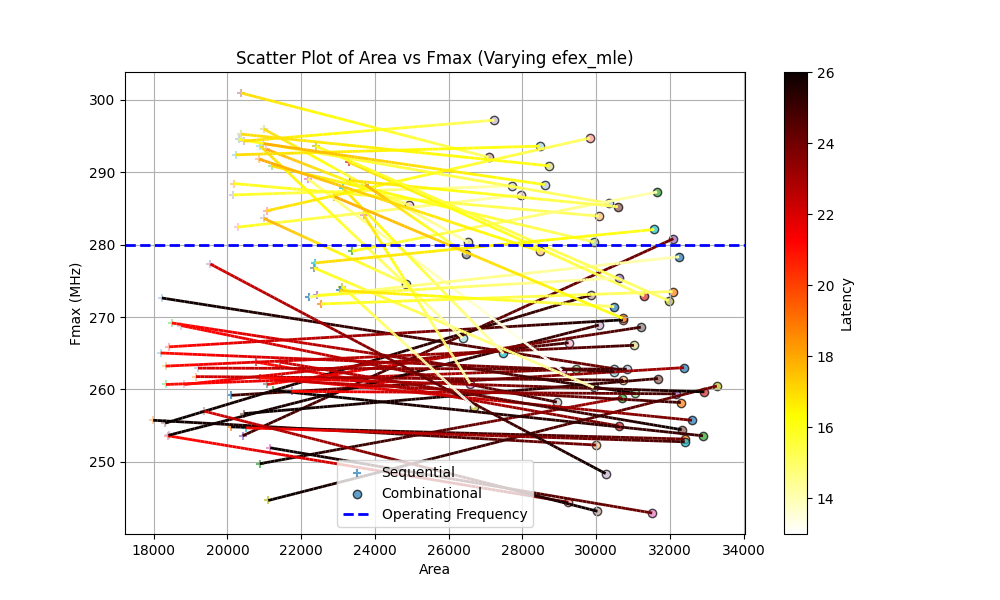
\includegraphics[trim={1cm 0 3cm 0}, clip, width=1\textwidth]{dse_efex_mle.png}
    \caption{Results when varying the CCORE type for the MLE}
    \label{fig:dse-efex-mle}    
    \centering
    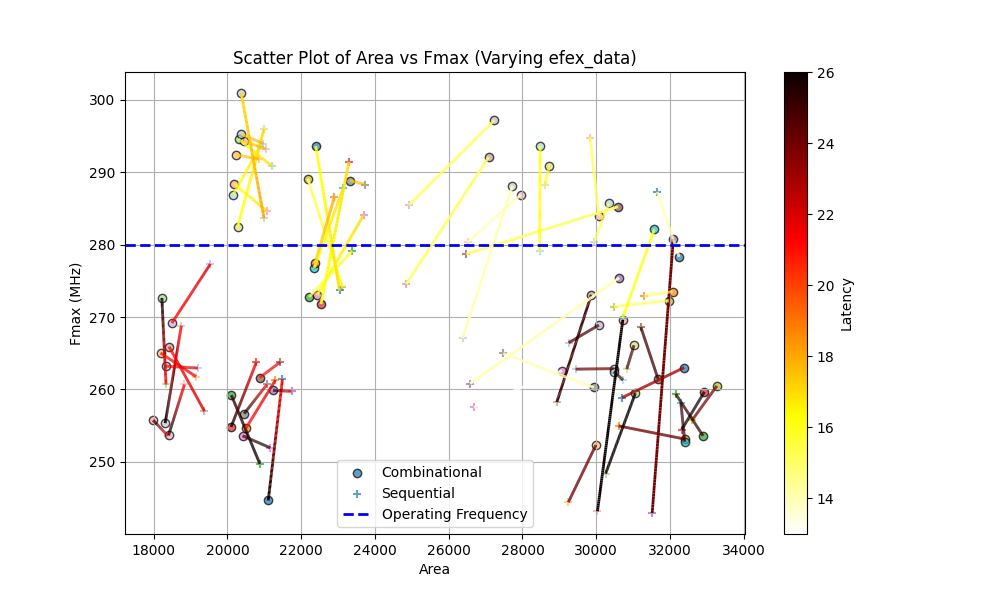
\includegraphics[trim={1cm 0 3cm 0}, clip, width=1\textwidth]{dse_efex_data.png}
    \caption{Results when varying the CCORE type for the Data Encoder}
    \label{fig:dse-efex-data}
\end{figure}
\begin{figure}
    \centering
    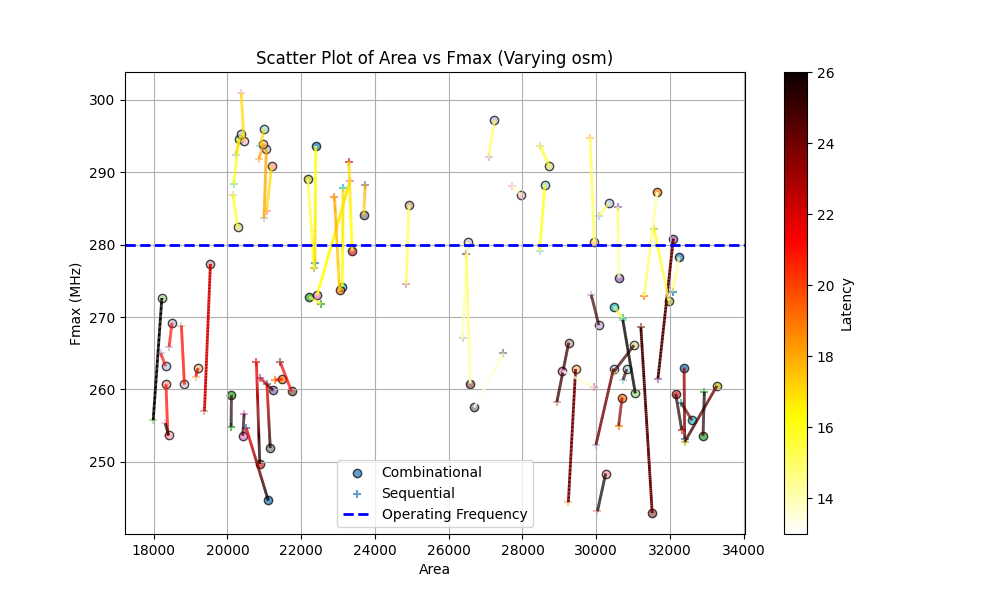
\includegraphics[trim={1cm 0 3cm 0}, clip, width=1\textwidth]{dse_osm.png}
    \caption{Results when varying the CCORE type for the OSM}
    \label{fig:dse-osm}
    \centering
    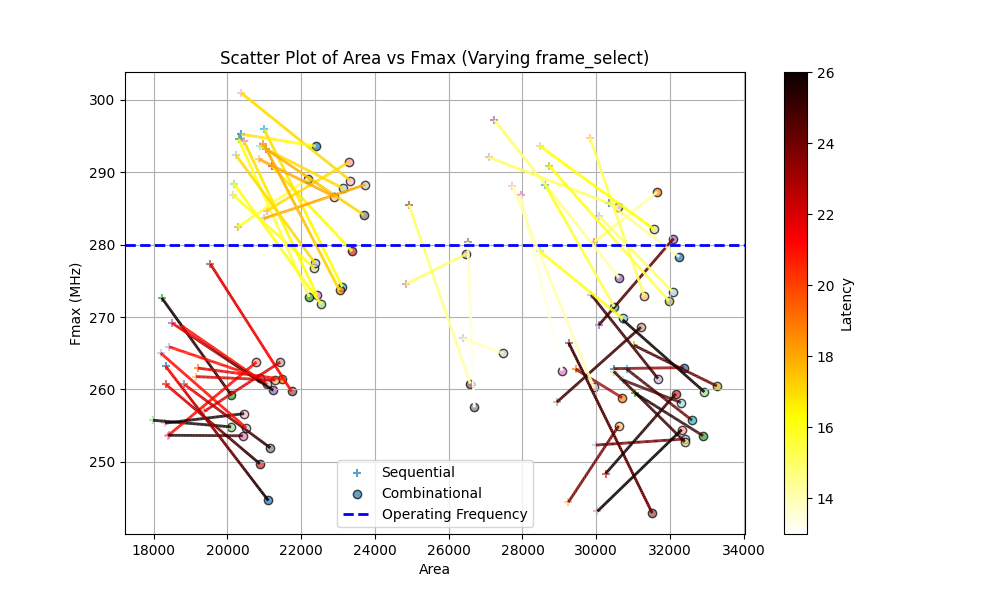
\includegraphics[trim={1cm 0 3cm 0}, clip, width=1\textwidth]{dse_frame_select.png}
    \caption{Results when varying the CCORE type for the Frame Select}
    \label{fig:dse-frame-select}
\end{figure}

Another interesting aspect rising from this DSE is the discrepancy between the results given by Catapult and the ones from Quartus. In the table below, the results are ordered by the area given by Catapult. The columns ``Goal'' to ``crc9'' contain the different CCORE options. ``mask.'' refers to the Masking block and is also called ``ena mux'',  ``emec'' refers to the EMEC Adapter, ``mle'' to the Multi Linear Encoder, ``frame'' to the Frame Encoder, ``osm'' to the Output Switch Matrix ``align.'' to the Frame Alignment and ``crc9'' to the Cyclic Redundant Check. Addtitionally, ``lat.'' refers to the latency. These abbreviations are used to fit the table in the page.

The colorization of the area values ranges from green when it is the lowest to red when it is the highest. The Quartus area values gradient follows the one from Catapult in average but for some groups of solutions Catapult seems to be too optimistic and for others too pessimistic. In the Catapult result, one can also see the slack column which indicates, in nanosecond, the time left for the design to meet the timing constraints. In most cases, Catapult is too optimistic, as the slack is positive but the \(F_{max}\) is under 280 MHz. 


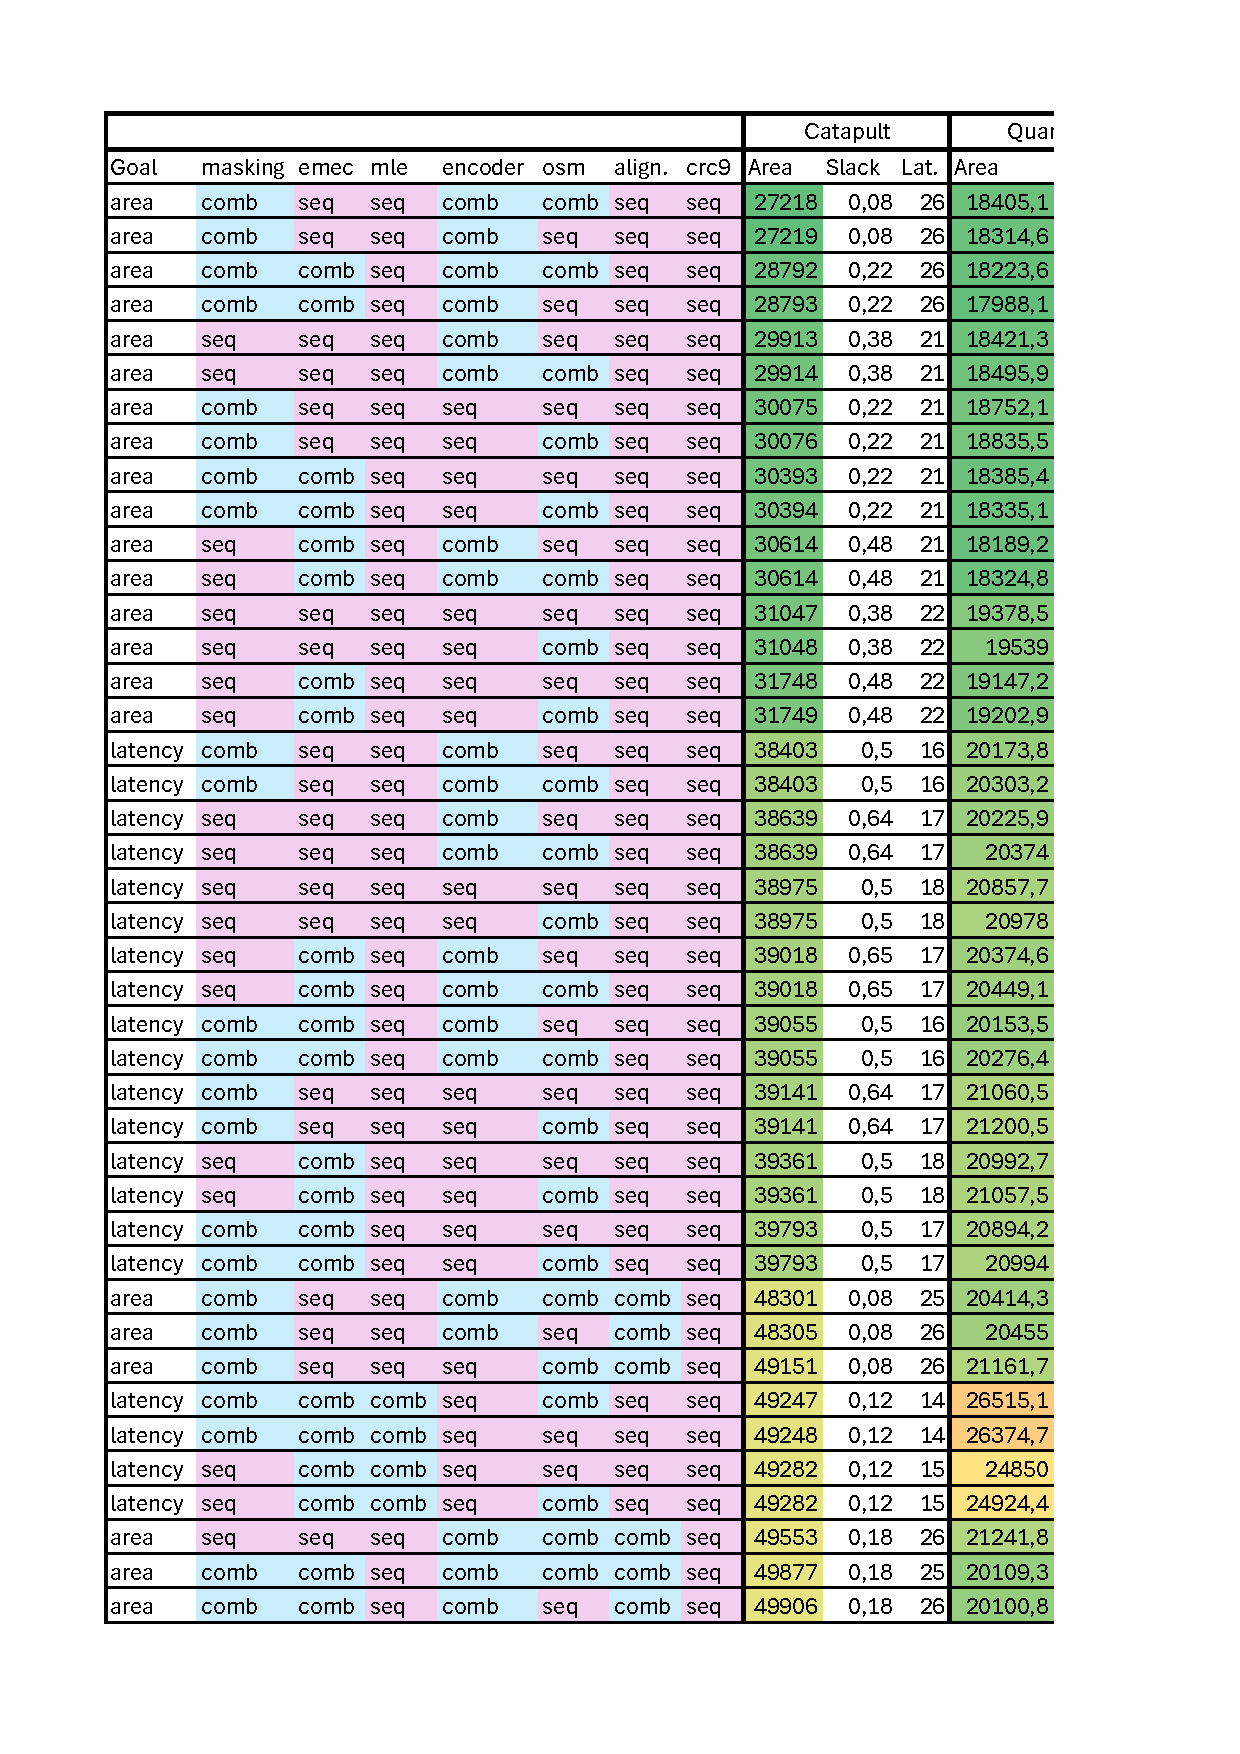
\includepdf[pages={1-},scale=0.25,width=1.3\textwidth,pagecommand={\null\vfill\captionof{table}{Compilation of the Design Space Exploration results}}]{../pdf/results.pdf}



%%%%%%%%%%%%%%%%%%%%%%%%%%%%%%%%%%%%%%%%%%%%%%%%%%%%%%%%%%%%%%%%%%%%%%%%%%%%%%%%
%%%%%%%%%%%%%%%%%%%%%%%%%%%%%%%%%%%%%%%%%%%%%%%%%%%%%%%%%%%%%%%%%%%%%%%%%%%%%%%%

\subsection{Unrolling inside or outside the CCORE}

%%%%%%%%%%%%%%%%%%%%%%%%%%%%%%%%%%%%%%%%%%%%%%%%%%%%%%%%%%%%%%%%%%%%%%%%%%%%%%%%

\subsubsection{Frame Alignment}

For the Frame Alignment, the v6 firmware unrolls outside of the CCORE. One frame alignment CCORE uses very little area, and because it uses only combinational logic, unrolling inside does not have any significant impact on the area. In table \ref{tab:frame-alignment-optimization}, we see that the first option yields a Frame Alignment of 21 ALMs. To compare it with the second option, we can multiply it by the number of instances that will be created: 48, for the 48 frames. This gives a total area of 1008, very similar to the 1087 of the second option. The \(F_{max}\) parameter, on the other hand, decreases by 98MHz, but this should be disregarded as the ``unrolling inside'' version of the CCORE contains the logic to synchronize the different instances, which the other one does not.

To have an idea of the true impact that the two implementations could have on the full firmware, the table \ref{tab:frame-alignment-optimization} also shows the area and \(F_{max}\) of the OSUM parent block. The low impact on the area is confirmed by our results, but the \(F_{max}\) gets a decrease of 3.6\%, reducing the margin of the design.

\begin{table}[ht]
    \centering
    \begin{tabular}{|c|c|c|}
        \hline
        \hline
        \multicolumn{3}{|c|}{unroll outside} \\
        \hline
        Block & Area (ALMs) & \(F_{max}\) (MHz) \\
        \hline
        Frame Alignment & \underline{21} (\(21\times48=1008\)) & 371.4 \\
        OSUM & 30449 & 274.5 \\
        \hline
        \hline
        \multicolumn{3}{|c|}{unroll inside} \\
        \hline
        Block & Area (ALMs) & \(F_{max}\) (MHz) \\
        \hline
        Frame Alignment & \underline{1087} (\(1087/48=22.6\))& 272.6\\
        OSUM & 30512 & 264.6\\
        \hline
    \end{tabular}
    \caption{Frame Alignment design exploration using the v6 firmware}
    \label{tab:frame-alignment-optimization}
\end{table}

In fact, unrolling outside can be useful when some sequential logic can be shared among all the CCOREs. The serialized Frame Alignment is a good example where unrolling outside has a positive impact, as it can be seen in the table \ref{tab:new-frame-alignment-optimization}. In this specific case, Catapult is able to optimize the design inside of the CCORE by sharing some logic between the different parallel instances. As a result, unrolling inside of the CCORE will create redundant logic and the total area of the CCORE instances is almost the double of the ``unrolling inside'' version. Additionally, this negative impact gets amplified on the OSUM block, with an area increase of 15\% and new timing violations with the ``unroll outside'' option.

\begin{table}[ht]
    \centering
    \begin{tabular}{|c|c|c|}
        \hline
        \hline
        \multicolumn{3}{|c|}{unroll outside} \\
        \hline
        Block & Area (ALMs) & \(F_{max}\) (MHz) \\
        \hline
        Frame Alignment & \underline{36} (\(36\times48=1728\)) & 388.8 \\
        OSUM & 18669 & \(274.7 < 280\) \\
        \hline
        \hline
        \multicolumn{3}{|c|}{unroll inside} \\
        \hline
        Block & Area (ALMs) & \(F_{max}\) (MHz) \\
        \hline
        Frame Alignment & \underline{940} (\(940/48=19.6\))& 345.1\\
        OSUM & 15875 & 291.1\\
        \hline
    \end{tabular}
    \caption{Frame Alignment design exploration using the new firmware}
    \label{tab:new-frame-alignment-optimization}
\end{table}

%%%%%%%%%%%%%%%%%%%%%%%%%%%%%%%%%%%%%%%%%%%%%%%%%%%%%%%%%%%%%%%%%%%%%%%%%%%%%%%%

\subsubsection{CRC9}

In the v6 firmware, similarly to the Frame Alignment, the CRC9 block is unrolled outside of the CCORE. The block alone represents 68 ALMs for an \(F_{max}\) of 395.6 MHz. When unrolling inside of the CCORE, the whole block gives an area of 3332 ALMs and an operating frequency of 357.1 MHz. Unrolling inside of the CCORE makes the block 49 times bigger, which matches the number of frames to process, and has a negative impact on the \(F_{max}\) which must be double checked in the OSUM block.

\begin{table}[ht]
    \centering
    \begin{tabular}{|c|c|c|}
        \hline
        \hline
        \multicolumn{3}{|c|}{unroll outside} \\
        \hline
        Block & Area (ALMs) & \(F_{max}\) (MHz) \\
        \hline
        CRC9 & \underline{68} (\(68\times48=3264\)) & 395.5 \\
        OSUM & 30534 & 271.89 \\
        \hline
        \hline
        \multicolumn{3}{|c|}{unroll inside} \\
        \hline
        Block & Area (ALMs) & \(F_{max}\) (MHz) \\
        \hline
        CRC9 & \underline{3332} (\(3332/48=69.4\))& 357.1\\
        OSUM & 30507 & 262.6\\
        \hline
    \end{tabular}
    \caption{CRC9 design exploration using the v6 firmware}
    \label{tab:crc9-optimization}
\end{table}

Table \ref{tab:crc9-optimization} shows the impact of both approaches on the OSUM block. While the area difference is negligeable, the \(F_{max}\) is reduced by 10 MHz when unrolling inside of the CCORE. 

%%%%%%%%%%%%%%%%%%%%%%%%%%%%%%%%%%%%%%%%%%%%%%%%%%%%%%%%%%%%%%%%%%%%%%%%%%%%%%%%
%%%%%%%%%%%%%%%%%%%%%%%%%%%%%%%%%%%%%%%%%%%%%%%%%%%%%%%%%%%%%%%%%%%%%%%%%%%%%%%%

\subsection{Overall Improvement}

